\chapter{Vorbetrachtungen}

Im folgenden werden die verwendeten Technologien betrachtet. Als Versionsverwaltungssoftware wurde Git\cite{git} auf der Platform Github\cite{github} verwendet, worauf nicht weiter eingegangen wird. Zum Erstellen der Simulation wurde Omnet++\cite{omnet} mithilfe des MiXiM-Frameworks\cite{mixim} benutzt.

\section{Evaluation von Systemen}

Im Entwicklungsprozess eines jeden Systems müssen neue Teile oder Module evaluiert werden. Für das Testen gibt es verschiedene Möglichkeiten, die einem zur Verfügung stehen. Im frühen Stadium der Entwicklung bietet das Abschätzen ohne Implementierung und daher ohne zu messen eine kostengünstige Variante zum Bestimmen von Designparametern. Allerdings sind diese Ergebnisse oftmals sehr grob und es lässt sich auch nicht jeder Wert so einfach bestimmen. \newline
Es ist daher notwendig genauere Tests durchzuführen. Wenn man ein komplett implementiertes und produziertes System anschließend testen möchte kann das sehr teuer werden, sollten viele Fehler auftreten oder wenn man merkt, dass die Implementierung wohl doch nicht die Optimale für ein gewünschtes Ziel ist. \newline
Man kann diesen Problemen zuvor kommen, indem man noch vor der ersten Implementierung eines Systems Simulationen und Emulationen erstellt und Prototypen anfertigt. Das senkt die Kosten mitunter erheblich und es lassen sich beinahe alle Parameter des zukünftigen Produkts überprüfen, auch wenn es das Testen des fertigen Produkts nicht komplett ersetzen kann.

\todo{überarbeiten}

\paragraph{Simulation}

Eine Simulation ist ein Modell eines Systems, welches dieses passend abbildet. Mit diesem Modell kann herausgefunden werden, was im realen System später umsetzbar ist. Der Zustand eines solchen Modells ändert sich im Laufe der (Simulations-)Zeit. Daher führt das Modell Zustandsübergange durch, welche als Events bezeichnet werden. Man kann Systeme nach den Zeitpunkten an denen Zustandswechsel möglich sind, in analoge und diskrete unterteilen. Wie der Name vermuten lässt können im analogen Fall zu jeder Zeit Zustandsübergänge stattfinden, im diskreten dagegen nur zu bestimmten Zeitpunkten.

\paragraph{Emulationen}

Eine Emulation ist die Implementierung eines Systems, welche den kompletten Funktionsumfang des Entwurfs abdeckt. Diese kann mit einer Hardwarebeschreibungssprache wie VHDL definiert werden und auf einem FPGA oder innerhalb eines Netzwerks von FPGAs ausgeführt werden. Man spricht daher von einer homogenen Hardwareplattform.

\paragraph{(Rapid) Prototyping}

Ein Prototyp ist ebenfalls eine Implementierung eines Systems, die den kompletten Funktionsumfang des Entwurfs abdeckt, allerdings geringere Anforderungen and Timing, Größe und Kosten stellt. Prototypen zum Beispiel oftmals wesentlich größer als das Endprodukt. Wenn er alle sonstigen Anforderungen zur Genüge erfüllt, so kann er in das finale Design umgewandelt werden und verliert bei diesem Prozess alle Grenzen des Prototyps. Im Gegensatz zur Emulation kommt eine heterogene Hardwareplattform zum Einsatz. So können etwa fertige Prozessoren, Speicher, weiterhin FPGAs oder spezielle Chips wie ein ASIC zum Einsatz kommen.

\endgraf

Für die Arbeit ist die Entscheidung auf eine Simulation gefallen. Man kann sich dabei auf die wesentlichen Funktionen konzentrieren und grundsätzliche Überlegungen über die genaue Umsetzung von gewissen Bauteilen zunächst außer Acht lassen. Ein Modell muss stets nur so genau spezifiziert werden wie nötig und so gut wie nie mit der Komplexität der Realität übereinstimmen. \newline
Der Fokus der Arbeit liegt daher auch auf dem Verwalten von Umweltparametern, der Erfassung dieser durch Sensoren auf vielen verschiedenen Sensorknoten und nicht darauf, wie die einzelnen Bauteile technisch aufgebaut sein könnten oder sollten. 

\section{Sensoren}

Den Hauptgegenstand in der Simulation bilden Sensoren, welche auf Sensorknoten angebracht sind. Ein solcher Knoten kann dann wiederum ein oder mehrere Sensoren besitzen.\newline
Sensoren sind das technische Gegenstück zu den menschlichen Sinnen, denn sie können physikalische oder chemische Eigenschaften wahrnehmen. Dabei arbeiten Sensoren allerdings noch wesentlich genauer, denn es lassen sich Messgrößen quantitativ exakt bestimmen.

\todo{ergänzen}

\begin{figure}[htbp]
\centering
\caption{Deutschlandkarte der mittleren Temperatur zwischen 1961 und 1990}
\label{fig:temperatur}
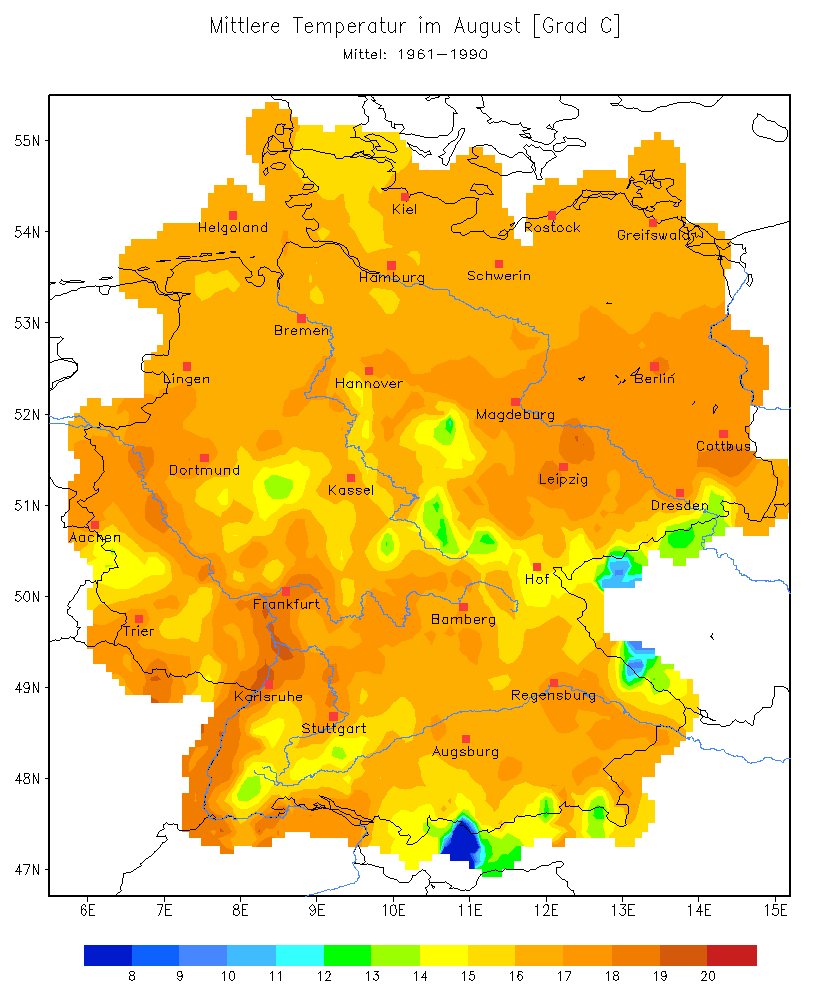
\includegraphics[width=\textwidth]{temperatur}
\end{figure}

\begin{figure}[htbp]
\centering
\caption{Deutschlandkarte: Beispielverteilung der Luftfeuchtigkeit}
\label{fig:feuchtigkeit}
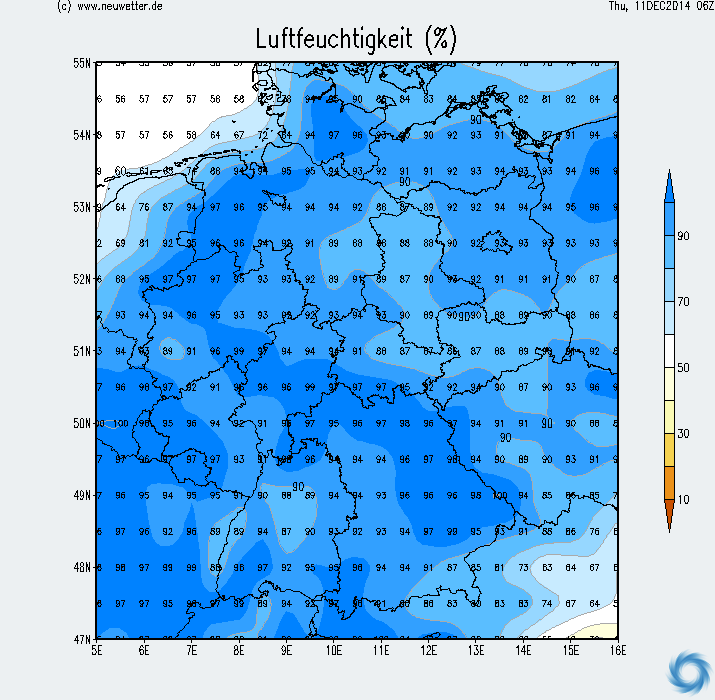
\includegraphics[width=\textwidth]{feuchtigkeit}
\end{figure}

\section{Sensornetzwerke}
\todo{ergänzen}
\section{Wake-up Receiver}

\todo{ergänzen}










